\باب{تقطیب موج}
اس باب میں \اصطلاح{تقطیب موج}\فرہنگ{تقطیب موج}\فرہنگ{موج!تقطیب}\حاشیہب{wave polarization}\فرہنگ{wave!polarization}  پر غور کیا جائے گا۔خطی تقطیب اور بیضوی تقطیب کے بعد دائری تقطیب پر تبصرہ کیا جائے گا۔

\حصہ{خطی، بیضوی اور دائری تقطیب}
اب تک اٹل سمت کے امواج پر غور کیا گیا۔یوں \عددیء{\az} جانب حرکت کرتا \عددیء{\ax} سمت کا میدان
\begin{align}
E_x = E_{x0} \cos (\omega t -\beta z)
\end{align}
لکھا گیا۔یہ مساوات خطی تقطیب کی مثال ہے جہاں میدان تمام اوقات صرف \عددیء{x} سمت میں پایا جاتا ہے۔عموماً \عددیء{\az} جانب حرکت کرتے موج میں \عددیء{\ax} کے علاوہ \عددیء{\ay} جزو بھی پایا جائے گا۔ایسی صورت میں موج کے اجزاء
\begin{gather}
\begin{aligned}\label{مساوات_قطبیت_عمومی_اجزاء}
E_x&=E_1 \cos (\omega t -\beta z)\\
E_y&=E_2 \cos (\omega t -\beta z -\delta)
\end{aligned}
\end{gather}
ہو سکتے ہیں جہاں دونوں اجزاء کے حیطے مختلف ممکن ہیں جبکہ ان میں زاویائی فاصلہ \عددیء{\delta} بھی پایا جا سکتا ہے۔ان اجزاء کا مجموعہ
\begin{align}\label{مساوات_قطبیت_عمومی_مساوات}
\kvec{E}=E_1 \cos (\omega t -\beta z) \ax+E_2 \cos (\omega t -\beta z -\delta) \ay
\end{align}
ایسی موج کو ظاہر کرے گا۔یہ مساوات غور طلب ہے۔آئیں خلاء میں کسی بھی اٹل نقطے پر وقت تبدیل ہونے سے  ایسی میدان پر غور کریں۔ہم خلاء میں  \عددیء{z=0} کو اٹل نقطہ لیتے ہوئے  میدان حاصل کرتے ہیں۔

\begin{figure}
\centering
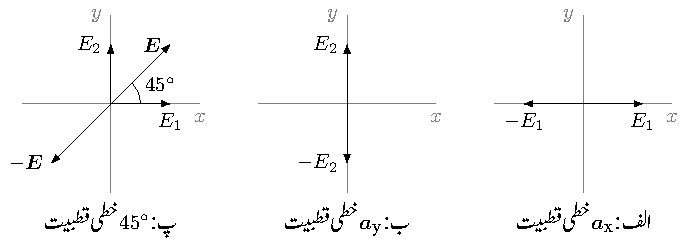
\includegraphics{figPolarizationFieldDirections}
\caption{خطی، دائری اور بیضوی قطبیت۔}
\label{شکل_قطبیت_خطی_قطبیت}
\end{figure}
اگر \عددیء{E_2=0} ہو تب وقت \عددیء{t} کے تبدیلی سے میدان کی قیمت \عددیء{-E_1\ax} تا \عددیء{+E_1\ax} تبدیل ہوتی ہے۔اس میدان کو تمام \عددیء{t} کے لئے شکل \حوالہ{شکل_قطبیت_خطی_قطبیت}-الف میں دکھایا گیا ہے۔آپ دیکھ سکتے ہیں کہ میدان کی نوک \عددیء{-E_1} تا \عددیء{+E_1} خطی لکیر پر رہتی ہے۔اسی حقیقت سے ایسے موج کی قطبیت کو \اصطلاح{خطی قطبیت}\فرہنگ{خطی!قطبیت}\فرہنگ{ْقطبیت!خطی}\حاشیہب{linear polarization}\فرہنگ{linear polarization}\فرہنگ{polarization!linear}\فرہنگ{linear!polarization}  کہتے ہیں۔یہ موج \عددیء{\ax} سمت میں خطی قطبیت رکھتی ہے۔اس کے برعکس اگر مساوات \حوالہ{مساوات_قطبیت_عمومی_مساوات} میں \عددیء{E_1=0} ہو تب یہ \عددیء{\ay} خطی قطبیت کی موج ہو گی جسے شکل \حوالہ{شکل_قطبیت_خطی_قطبیت}-ب میں دکھایا گیا ہے۔اگر \عددیء{E_1=E_2=E_{12}} اور \عددیء{\delta=0} ہوں تب بھی خطی قطبیت کی موج حاصل ہوتی ہے البتہ یہ موج افقی محدد کے ساتھ \عددیء{45^\circ} کا زاویہ بناتی ہے۔شکل \حوالہ{شکل_قطبیت_خطی_قطبیت}-پ میں اس موج کو دکھایا گیا ہے۔

آئیں اب ذرہ دلچسپ صورت حال دیکھیں۔نقطہ \عددیء{z=0} پر مساوات \حوالہ{مساوات_قطبیت_عمومی_اجزاء}
\begin{gather}
\begin{aligned}\label{مساوات_قطبیت_ابتدائی_نقطے_پر_میدان}
E_x&=E_1 \cos \omega t\\
E_y&=E_2 \cos (\omega t  -\delta)
\end{aligned}
\end{gather}
صورت اختیار کر لیتے ہیں جس میں \عددیء{E_y} کو
\begin{align*}
E_y=E_2 \left(\cos \omega t \cos \delta + \sin \omega t \sin \delta\right)
\end{align*}
لکھنا ممکن ہے۔اس مساوات میں،  \عددیء{E_x} کی مساوات استعمال کرتے ہوئے،  \عددیء{\cos \omega t =\tfrac{E_x}{E_1}} اور \عددیء{\sin \omega t=\sqrt{1-\left(\tfrac{E_x}{E_1} \right)^2}} پر کر کے
\begin{align*}
E_y=E_2 \left[\frac{E_x}{E_1} \cos \delta+\sqrt{1-\left(\frac{E_x}{E_1}\right)^2} \sin \delta\right]
\end{align*}
ملتا ہے جسے
\begin{align}\label{مساوات_قطبیت_عمومی_بیضوی_قطبیت_الف}
\frac{E_x^2}{E_1^2}-2 \frac{E_x}{E_1} \frac{E_y}{E_2} \cos \delta +\frac{E_y^2}{E_2^2}=\sin^2 \delta
\end{align}
یا
\begin{align}\label{مساوات_قطبیت_عمومی_بیضوی_قطبیت_ب}
a E_x^2-b E_x E_y +c E_y^2=1
\end{align}
لکھا جا سکتا ہے جہاں
\begin{align}
a=\frac{1}{E_1^2 \sin^2 \delta} \quad \quad b=\frac{2 \cos \delta}{E_1 E_2 \sin^2 \delta} \quad \quad c=\frac{1}{E_2^2 \sin^2 \delta}
\end{align}
لئے گئے ہیں۔مساوات \حوالہ{مساوات_قطبیت_عمومی_بیضوی_قطبیت_ب} \اصطلاح{بیضوی قطبیت}\فرہنگ{قطبیت!بیضوی}\فرہنگ{بیضوی قطبیت}\حاشیہب{elliptic polarization}\فرہنگ{elliptic!polarization}\فرہنگ{polarization!elliptic} کی عمومی مساوات ہے۔

مساوات \حوالہ{مساوات_قطبیت_عمومی_بیضوی_قطبیت_الف} میں \عددیء{E_1=E_2=E_{0}} اور \عددیء{\delta=\mp 90^\circ} کی صورت میں
\begin{align}\label{مساوات_قطبیت_عمومی_دائری_قطبیت}
E_x^2 +E_y^2=E_{0}^2
\end{align}
حاصل ہوتا ہے جو دائرے کی مساوات ہے اور جسے شکل \حوالہ{شکل_قطبیت_دائری_اور_بیضوی_قطبیت}-الف میں دکھایا گیا ہے۔شکل میں \عددیء{E_1} اور \عددیء{E_2} بھی ظاہر کئے گئے ہیں جن کی لمبائی برابر ہے۔مساوات \حوالہ{مساوات_قطبیت_ابتدائی_نقطے_پر_میدان} سے \عددیء{\delta=+90^\circ} کی صورت میں \عددیء{\omega t=0} پر 
\begin{align*}
E_x&=E_{0} \cos 0=E_{0}\\  
E_y&=E_{0} \cos (0  -90^\circ) =0  \quad \quad (\delta =+90^\circ)
\end{align*}
حاصل ہوتے ہیں جبکہ کچھ ہی لمحے بعد \عددیء{\omega t =30^\circ} کی صورت میں
\begin{align*}
E_x&=E_{0} \cos 30^\circ=0.866 E_{0} \\
E_y&=E_{0} \cos (30^\circ  -90^\circ) =0.5 E_{0} \quad \quad (\delta =+90^\circ)
\end{align*}
حاصل ہوتا ہے۔شکل \حوالہ{شکل_قطبیت_دایاں_بایاں_ہاتھ_دائری}-الف میں دونوں اوقات پر موج دکھائی گئی ہے۔آپ دیکھ سکتے ہیں کہ بڑھتے وقت کے ساتھ میدان کی نوک دائرے پر گھڑی کے الٹ سمت میں حرکت کرتی ہے۔اس شکل میں موج کے حرکت کی سمت \عددیء{\az} کاغذ سے باہر کو ہے۔اگر دائیں ہاتھ کے انگوٹھے کو موج کے حرکت کی سمت میں رکھا جائے تو اس ہاتھ کی بقایا چار انگلیاں دائرے پر میدان کی نوک کی حرکت کا سمت دیتی ہیں۔یوں \عددیء{\delta=+90^\circ} کی صورت میں مساوات \حوالہ{مساوات_قطبیت_عمومی_دائری_قطبیت} \اصطلاح{دائیں دائری قطبیت}\فرہنگ{دایاں دائری قطبیت}\فرہنگ{قطبیت!دایاں دائری}\حاشیہب{right circular polarization}\فرہنگ{right circular polarization}\فرہنگ{polarization!right circular} کی موج کو ظاہر کرتا ہے۔   
\begin{figure}
\centering
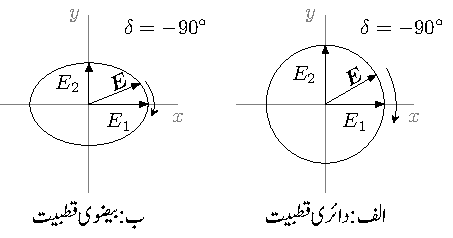
\includegraphics{figPolarizationCircularAndElliptic}
\caption{دائری اور بیضوی قطبیت۔}
\label{شکل_قطبیت_دائری_اور_بیضوی_قطبیت}
\end{figure}

اسی طرح \عددیء{\delta=-90^\circ} کی صورت میں \اصطلاح{بائیں دائری قطبیت}\فرہنگ{قطبیت!بائیں دائری}\حاشیہب{left circular polarization}\فرہنگ{left circular polarization} حاصل ہوتی ہے جسے شکل \حوالہ{شکل_قطبیت_دایاں_بایاں_ہاتھ_دائری}-ب میں دکھایا گیا ہے۔

دائیں ہاتھ قطبی موج سے مراد وہ موج ہے جو آپ کی طرف حرکت کرتے ہوئے آپ کو دائیں ہاتھ گھومتی نظر آئے۔کسی موج کی قطبیت سے مراد وہ قطبیت ہے جو دیکھنے والے کی طرف حرکت کرتی موج کی قطبیت ہو گی۔

جہاں بھی غلطی کی گنجائش ہو وہاں بہتر ہوتا ہے کہ قطبیت کا ذکر کرتے وقت حرکت کی سمت کا بھی ذکر کیا جائے۔

\begin{figure}
\centering
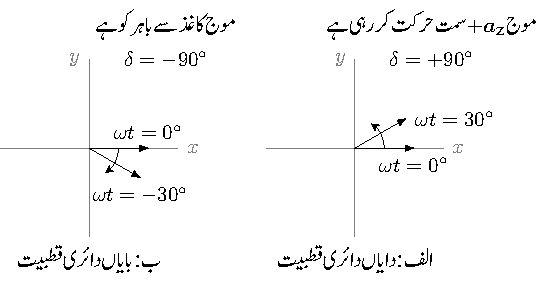
\includegraphics{figPolarizationRightAndLeftCircularPolarizeds}
\caption{دائیں ہاتھ اور بائیں ہاتھ کی دائری قطبیت۔}
\label{شکل_قطبیت_دایاں_بایاں_ہاتھ_دائری}
\end{figure}

مساوات \حوالہ{مساوات_قطبیت_عمومی_بیضوی_قطبیت_الف} میں \عددیء{E_1 \ne E_2} کی صورت میں بیضوی موج حاصل ہوتی ہے جسے شکل \حوالہ{شکل_قطبیت_دائری_اور_بیضوی_قطبیت}-ب میں دکھایا گیا ہے۔

شکل \حوالہ{شکل_قطبیت_عمومی_بیضوی} میں مساوات \حوالہ{مساوات_قطبیت_عمومی_بیضوی_قطبیت_ب} کی عمومی شکل دکھائی گئی ہے۔
\begin{figure}
\centering
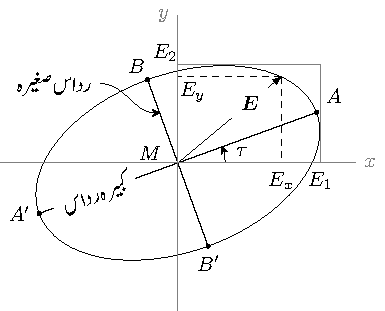
\includegraphics{figPolarizationEllipticAtAngle}
\caption{عمومی بیضوی قطبیت۔}
\label{شکل_قطبیت_عمومی_بیضوی}
\end{figure}
اس شکل میں \اصطلاح{ترخیم}\فرہنگ{ترخیم}\حاشیہب{ellipse}\فرہنگ{ellipse} افقی محدد کے ساتھ \عددیء{\tau} زاویہ بناتا ہے لہٰذا یہ \عددیء{\tau} زاویے کی بیضوی قطبیت کو ظاہر کرتی ہے۔

\حصہ{بیضوی یا دائری قطبی امواج کا پوئنٹنگ سمتیہ}
کسی بھی موج کی اوسط طاقت مساوات \حوالہ{مساوات_موج_مخلوط_پوئنٹنگ_سمتیہ}
\begin{align*}
\pmb{\mathscr{P}}_{\text{اوسط}}=\frac{1}{2}\left[\kvec{E}_s \times \kvec{H}_s^* \right]_{\text{حقیقی}}
\end{align*}
سے حاصل کی جا سکتی ہے۔شکل \حوالہ{شکل_قطبیت_عمومی_بیضوی} کے عمومی بیضوی قطبی موج کے \عددی{x} اور \عددیء{y} اجزاء
\begin{align}
E_{sx}&=E_1 e^{j(\omega t -\beta z)} \label{مساوات_تقطیب_عمومی_بیضوی_برقی_الف}\\
E_{sy}&=E_2 e^{j(\omega t -\beta z +\delta)}\label{مساوات_تقطیب_عمومی_بیضوی_برقی_ب}
\end{align}
میں \عددیء{\delta} زاویائی فرق پایا جاتا ہے۔کسی بھی نقطے پر کل برقی میدان ان اجزاء کا سمتی مجموعہ ہو گا جسے نقطہ \عددیء{z=0} پر 
\begin{align}
\kvec{E}_s =\ax E_1 e^{j \omega t}+\ay E_2 e^{j(\omega t +\delta)}
\end{align}
لکھا جا سکتا ہے۔چونکہ
\begin{align*}
\frac{\kvec{E}}{\kvec{H}}=\eta=\abs{\eta}e^{j \theta_{\eta}}
\end{align*}
ہوتا ہے لہٰذا مساوات \حوالہ{مساوات_تقطیب_عمومی_بیضوی_برقی_الف} کی جوڑی مقناطیسی موج
\begin{align*}
H_{sy}=\frac{E_{sx}}{\abs{\eta}} e^{-j \theta_{\eta}}=\frac{E_1}{\abs{\eta}} e^{j(\omega t -\beta z-\theta_{\eta})}=H_1 e^{j(\omega t -\beta z-\theta_{\eta})}
\end{align*}
ہو گی۔اسی طرح مساوات \حوالہ{مساوات_تقطیب_عمومی_بیضوی_برقی_ب} کی جوڑی
\begin{align}
H_{sx}=-H_2 e^{j(\omega t -\beta z+\delta-\theta_{\eta})}
\end{align}
ہو گی۔کسی بھی نقطے پر مقناطیسی میدان ان اجزاء کا سمتی مجموعہ ہو گا جسے نقطہ \عددیء{z=0} پر
\begin{align}
\kvec{H}_s=-\ax H_2 e^{j(\omega t +\delta-\theta_{\eta})}+\ay H_1 e^{j(\omega t -\theta_{\eta})}
\end{align}
لکھا جا سکتا ہے۔
ہو گا۔جوڑی دار مخلوط \عددیء{\kvec{H}_s} کی قیمت مندرجہ بالا مساوات میں مثبت \عددیء{j} کو منفی اور منفی \عددیء{j} کو مثبت لکھ کر حاصل ہوتا ہے یعنی
\begin{align}
\kvec{H}_s^*=-\ax H_2 e^{-j(\omega t +\delta-\theta_{\eta})}+\ay H_1 e^{-j(\omega t -\theta_{\eta})}
\end{align}
مخلوط پوئنٹنگ سمتیہ سے اوسط طاقت
\begin{align*}
\pmb{\mathscr{P}}_{\text{اوسط}}&=\frac{1}{2}\left[\left(\ax E_1 e^{j \omega t}+\ay E_2 e^{j(\omega t +\delta)}\right) \times \left(-\ax H_2 e^{-j(\omega t +\delta-\theta_{\eta})}+\ay H_1 e^{-j(\omega t -\theta_{\eta})}\right) \right]_{\text{حقیقی}}\\
&=\frac{1}{2} \az \left[E_1 H_1 e^{j\theta_{\eta}}+E_2 H_2 e^{j \theta_{\eta}} \right]_{\text{حقیقی}}
\end{align*}
یعنی
\begin{align}
\pmb{\mathscr{P}}_{\text{اوسط}}&=\frac{1}{2} \az \left(E_1 H_1+E_2 H_2 \right) \cos \theta_{\eta}
\end{align}
حاصل ہوتی ہے۔آپ دیکھ سکتے ہیں کہ طاقت \عددیء{\delta} پر بالکل منحصر نہیں ہے۔

بے ضیاع خطے میں برقی اور مقناطیسی میدان ہم قدم ہوتے ہیں۔ان میں \عددیء{\tfrac{E_1}{H_1}=\tfrac{E_2}{H_2}=\eta_0} کے برابر ہوتا ہے جہاں حقیقی قدرتی رکاوٹ کا زاویہ  \عددیء{\theta_{\eta}=0} ہے۔ایسے خطے میں
\begin{gather}
\begin{aligned}
\pmb{\mathscr{P}}_{\text{اوسط}}&=\frac{1}{2} \az \left(E_1 H_1+E_2 H_2 \right)\\
&=\frac{1}{2}\az \left(H_1^2+H_2^2 \right) \eta_0=\frac{1}{2}\az H^2 \eta_0
\end{aligned}
\end{gather}
ہو گا جہاں \عددیء{H=\sqrt{H_1^2+H_2^2}} کے برابر ہے۔اس مساوات کو 
\begin{gather}
\begin{aligned}\label{مساوات_تقطیب_اوسط_طاقت_برقی_میدان_معلوم}
\pmb{\mathscr{P}}_{\text{اوسط}}&=\frac{1}{2} \az \left(E_1 H_1+E_2 H_2 \right)\\
&=\frac{1}{2}\az \frac{E_1^2+E_2^2}{\eta_0}=\frac{1}{2}\az \frac{E^2}{\eta_0}
\end{aligned}
\end{gather}
بھی لکھا جا سکتا ہے جہاں \عددیء{E=\sqrt{E_1^2+E_2^2}} کے برابر ہے۔
%============
\ابتدا{مثال}
خلاء میں بیضوی قطبی موج کے اجزاء
\begin{align*}
E_x&=2 \cos (\omega t -\beta z)\\
E_y&=3 \cos (\omega t -\beta z+75^{\circ})
\end{align*}
وولٹ فی میٹر ہیں۔موج کی فی مربع میٹر اوسط طاقت دریافت کریں۔

حل:خالی خلاء کی قدرتی رکاوٹ \عددیء{\eta=120\pi} لیتے ہوئے مساوات \حوالہ{مساوات_تقطیب_اوسط_طاقت_برقی_میدان_معلوم}
سے
\begin{align*}
\mathscr{P}_{\text{اوسط}}&=\frac{1}{2} \frac{2^2+3^2}{120\pi}=\SI{17.24}{\milli \watt \per \meter \squared}
\end{align*}
حاصل ہوتا ہے۔
\انتہا{مثال}
%================
